%%%%%%%%%%%%%%%%%%%%%%%%%%%%%%%%%%%%%%%%%%%%%%%%%%%%%%%%%%%%%%%%%%%%%%%%%%%%
\def\TITLE{\bfseries $\boldsymbol{SU(2)}$からKac-Moody代数に至る道}
\def\AUTHOR{黒木玄}
\def\DATE{2017年6月1日(木)\\
\href
{https://mathtod.online/@genkuroki/204074}
{https://mathtod.online/@genkuroki/204074}
}
\def\PDFTITLE{表現論入門}
\def\PDFAUTHOR{黒木玄}
\def\PDFSUBJECT{表現論}
%%%%%%%%%%%%%%%%%%%%%%%%%%%%%%%%%%%%%%%%%%%%%%%%%%%%%%%%%%%%%%%%%%%%%%%%%%%%
\documentclass[12pt,twoside]{jarticle}
\usepackage{amsmath,amssymb,amsthm}
%%%%%%%%%%%%%%%%%%%%%%%%%%%%%%%%%%%%%%%%%%%%%%%%%%%%%%%%%%%%%%%%%%%%%%%%%%%%%%
%\usepackage{hyperref}
\usepackage[dvipdfmx]{hyperref}
\usepackage{pxjahyper}
\hypersetup{%
 bookmarksnumbered=true,%
 colorlinks=true,%
 setpagesize=false,%
 pdftitle={\PDFTITLE},%
 pdfauthor={\PDFAUTHOR},%
 pdfsubject={\PDFSUBJECT},%
 pdfkeywords={TeX; dvipdfmx; hyperref; color;}}
\newcommand\arxivref[1]{\href{http://arxiv.org/abs/#1}{\tt arXiv:#1}}
\newcommand\TILDE{\textasciitilde}
\newcommand\US{\textunderscore}
%%%%%%%%%%%%%%%%%%%%%%%%%%%%%%%%%%%%%%%%%%%%%%%%%%%%%%%%%%%%%%%%%%%%%%%%%%%%%%
\usepackage[dvipdfmx]{graphicx}
\usepackage[all]{xy}
%%%%%%%%%%%%%%%%%%%%%%%%%%%%%%%%%%%%%%%%%%%%%%%%%%%%%%%%%%%%%%%%%%%%%%%%%%%%%%
\usepackage[dvipdfmx]{color}
\newcommand\red{\color{red}}
\newcommand\blue{\color{blue}}
\newcommand\green{\color{green}}
\newcommand\magenta{\color{magenta}}
\newcommand\cyan{\color{cyan}}
\newcommand\yellow{\color{yellow}}
\newcommand\white{\color{white}}
\newcommand\black{\color{black}}
\renewcommand\r{\red}
\renewcommand\b{\blue}
%%%%%%%%%%%%%%%%%%%%%%%%%%%%%%%%%%%%%%%%%%%%%%%%%%%%%%%%%%%%%%%%%%%%%%%%%%%%%%
\pagestyle{headings}
\setlength{\oddsidemargin}{0cm}
\setlength{\evensidemargin}{0cm}
\setlength{\topmargin}{-1.3cm}
\setlength{\textheight}{25cm}
\setlength{\textwidth}{16cm}
%\allowdisplaybreaks
%%%%%%%%%%%%%%%%%%%%%%%%%%%%%%%%%%%%%%%%%%%%%%%%%%%%%%%%%%%%%%%%%%%%%%%%%%%%
%\newcommand\N{{\mathbb N}} % natural numbers
\newcommand\Z{{\mathbb Z}} % rational integers
\newcommand\F{{\mathbb F}} % finite field
\newcommand\Q{{\mathbb Q}} % rational numbers
\newcommand\R{{\mathbb R}} % real numbers
\newcommand\C{{\mathbb C}} % complex numbers
%\renewcommand\P{{\mathbb P}} % projective spaces
\newcommand\eps{\varepsilon}
\renewcommand\d{\partial}
\renewcommand\Re{\operatorname{Re}}
\renewcommand\Im{\operatorname{Im}}
\newcommand\bra{\langle}
\newcommand\ket{\rangle}
\renewcommand\setminus{\smallsetminus}
\newcommand\Hom{\operatorname{Hom}}
\newcommand\Aut{\operatorname{Aut}}
\newcommand\End{\operatorname{End}}
\newcommand\diag{\operatorname{diag}}
\newcommand\su{\operatorname{su}}
\newcommand\sltwo{\operatorname{sl}_2(\C)}
\newcommand\ad{\operatorname{ad}}
%%%%%%%%%%%%%%%%%%%%%%%%%%%%%%%%%%%%%%%%%%%%%%%%%%%%%%%%%%%%%%%%%%%%%%%%%%%%
%
% enumerate
%
\renewcommand\labelenumi{(\arabic{enumi})}
\renewcommand\labelenumii{(\alph{enumii})}
\renewcommand\labelenumiii{(\roman{enumiii})}
%%%%%%%%%%%%%%%%%%%%%%%%%%%%%%%%%%%%%%%%%%%%%%%%%%%%%%%%%%%%%%%%%%%%%%%%%%%%
%
% 定理環境
%
\newtheoremstyle{jplain}% name
{}% space above
{}% space below
{\normalfont}% body  font
{}% indent amount
{\bfseries}% theorem head font
{.}% punctuation after theorem head
{4pt}% space after theorem head (default: 5pt)
{\thmname{#1}\thmnumber{#2}\thmnote{\hspace{2pt}(#3)}}% theorem head spec

%\theoremstyle{plain} % 見出しをボールド, 本文で斜体を使う
%\theoremstyle{definition} % 見出しをボールド, 本文で斜体を使わない
\theoremstyle{jplain}
\newtheorem{theorem}{定理}
\newtheorem*{theorem*}{定理} % 番号を付けない
\newtheorem{prop}[theorem]{命題}
\newtheorem*{prop*}{命題}
\newtheorem{lemma}[theorem]{補題}
\newtheorem*{lemma*}{補題}
\newtheorem{cor}[theorem]{系}
\newtheorem*{cor*}{系}
\newtheorem{example}[theorem]{例}
\newtheorem*{example*}{例}
\newtheorem{axiom}[theorem]{公理}
\newtheorem*{axiom*}{公理}
\newtheorem{problem}[theorem]{問題}
\newtheorem*{problem*}{問題}
\newtheorem{summary}[theorem]{要約}
\newtheorem*{summary*}{要約}
\newtheorem{guide}[theorem]{参考}
\newtheorem*{guide*}{参考}
%
%\theoremstyle{definition} % 見出しをボールド, 本文で斜体を使わない
\theoremstyle{jplain}
\newtheorem{definition}[theorem]{定義}
\newtheorem*{definition*}{定義} % 番号を付けない
%
%\theoremstyle{remark} % 見出しをイタリック, 本文で斜体を使わない
%\theoremstyle{definition} % 見出しをボールド, 本文で斜体を使わない
\theoremstyle{jplain}
\newtheorem{remark}[theorem]{注意}
\newtheorem*{remark*}{注意}
%
\numberwithin{theorem}{section}
\numberwithin{equation}{section}
\numberwithin{figure}{section}
\numberwithin{table}{section}
%
% 引用コマンド
%
\newcommand\secref[1]{第\ref{#1}節}
\newcommand\theoremref[1]{定理\ref{#1}}
\newcommand\propref[1]{命題\ref{#1}}
\newcommand\lemmaref[1]{補題\ref{#1}}
\newcommand\corref[1]{系\ref{#1}}
\newcommand\exampleref[1]{例\ref{#1}}
\newcommand\axiomref[1]{公理\ref{#1}}
\newcommand\problemref[1]{問題\ref{#1}}
\newcommand\summaryref[1]{要約\ref{#1}}
\newcommand\guideref[1]{参考\ref{#1}}
\newcommand\definitionref[1]{定義\ref{#1}}
\newcommand\remarkref[1]{注意\ref{#1}}
%
\newcommand\figureref[1]{図\ref{#1}}
\newcommand\tableref[1]{表\ref{#1}}
\newcommand\fnref[1]{脚注\ref{#1}}
%
% \qed を自動で入れない proof 環境を再定義
%
\makeatletter
\renewenvironment{proof}[1][\proofname]{\par
%\newenvironment{Proof}[1][\Proofname]{\par
  \normalfont
  \topsep6\p@\@plus6\p@ \trivlist
  \item[\hskip\labelsep{\bfseries #1}\@addpunct{\bfseries.}]\ignorespaces
}{%
  \endtrivlist
}
\renewcommand{\proofname}{証明}
%\newcommand{\Proofname}{証明}
\makeatother
%
% 正方形の \qed を長方形に再定義
%
\makeatletter
\def\BOXSYMBOL{\RIfM@\bgroup\else$\bgroup\aftergroup$\fi
  \vcenter{\hrule\hbox{\vrule height.85em\kern.6em\vrule}\hrule}\egroup}
\makeatother
\newcommand{\BOX}{%
  \ifmmode\else\leavevmode\unskip\penalty9999\hbox{}\nobreak\hfill\fi
  \quad\hbox{\BOXSYMBOL}}
\renewcommand\qed{\BOX}
%\newcommand\QED{\BOX}
%%%%%%%%%%%%%%%%%%%%%%%%%%%%%%%%%%%%%%%%%%%%%%%%%%%%%%%%%%%%%%%%%%%%%%%%%%%%
\begin{document}
%%%%%%%%%%%%%%%%%%%%%%%%%%%%%%%%%%%%%%%%%%%%%%%%%%%%%%%%%%%%%%%%%%%%%%%%%%%%
\title{\TITLE}
\author{\AUTHOR}
\date{\DATE}
\maketitle
%\tableofcontents
%%%%%%%%%%%%%%%%%%%%%%%%%%%%%%%%%%%%%%%%%%%%%%%%%%%%%%%%%%%%%%%%%%%%%%%%%%%%
%\setcounter{section}{-1} % 最初の節番号を0にする

\section{ May 31, 2017 10:56am}








黒木玄 Gen Kuroki
@genkuroki

\href
{https://mathtod.online/@7shi/203900}
{https://mathtod.online/@7shi/203900}

四元数と3次元の回転の関係は「Lie群 $SU(2)$ の随伴表現」. $i,j,k$ を正規直交基底とする3次元Euclid空間に $i,j,k$ 軸を中心とする角度 $2\theta$ の回転がそれぞれ\begin{align*}&a\mapsto e^{i\theta}a e^{-i\theta},\\ &a\mapsto e^{j\theta}a e^{-j\theta},\\ &a\mapsto e^{k\theta}a e^{-k\theta}\end{align*}で作用している. Lie群 $SU(2)$ の四元数体 $\mathbb H$ を使った実現の仕方は\begin{align*}SU(2)=\{\,g\in\mathbb H\mid |g|=1\,\}.\end{align*}これのLie代数が\begin{align*}\operatorname{su}(2)=\mathbb Ri+\mathbb Rj+\mathbb Rk.\end{align*}$SU(2)$ の $\operatorname{su}(2)$ への随伴表現の特殊化が上で示した式. 







\section{ May 31, 2017  9:31pm}








黒木玄 Gen Kuroki
@genkuroki


複素数(実数と $i$ から生成される)を実2次正方行列によって\begin{align*}i\mapsto\begin{bmatrix}0&-1\\ 1&0\end{bmatrix}\end{align*}と実現できることはよく知られている. 四元数(実数と $i,j$ から生成される)も次によって複素2次正方行列で実現できる:\begin{align*}i\mapsto\begin{bmatrix}i&0\\ 0&-i\end{bmatrix},\\ j\mapsto\begin{bmatrix}0&-1\\ 1&0\end{bmatrix}.\end{align*}すなわち複素数 $z,w$ に対して\begin{align*}z+jw\mapsto\begin{bmatrix}z&-\overline{w}\\ w&\overline{z}\end{bmatrix}.\end{align*}四元数はこの形の複素2次正方行列のことだと思ってよい. 







\section{ May 31, 2017  9:46pm}








黒木玄 Gen Kuroki
@genkuroki


複素 $n$ 次正方行列全体の集合を $M_n(\mathbb C)$ と書く. 行列の積に関する群 $SU(n)$ は\begin{align*}SU(n)=\{\, A\in M_n(\mathbb C)\mid A^*A=AA^*=E, |A|=1\,\}\end{align*}と定義される. $SU(2)$ については\begin{align*}SU(2)=\left\{\,\left.\begin{bmatrix}z&-\overline{w}\\ w&\overline{z}\end{bmatrix}\in M_2(\mathbb C)\,\right|\,|z|^2+|w|^2=1\,\right\}.\end{align*}この式から $SU(2)$ は絶対値が $1$ の四元数全体のなす群と同一視できることや, $SU(2)$ は3次元球面 $|z|^2+|w|^2=1$ になっていることもわかります. 

四元数, 複素2次正方行列, 3次元球面などなどの風景は基本的かつ様々に一般化されるので一度は見ておいて損がないです. 







\section{ May 31, 2017 10:06pm}








黒木玄 Gen Kuroki
@genkuroki


行列群 $SU(n)$ のLie代数 $\su(n)$ の定義はその単位元 $E$ での接空間です. 計算すると\begin{align*}\su(n)=\{\,X\in M_n(\mathbb C)\mid X+X^*=0, \operatorname{tr}X=0\,\}.\end{align*}接空間の定義を知らない人はこれを定義だと思ってもよいです. そして $X,Y\in\su(n)$ ならば\begin{align*}[X,Y]=XY-YX\in\su(n),\\ e^X=\sum_{n=0}^\infty x^n/n!\in SU(n)\end{align*}となることも容易に確認できます. $\su(2)$ が実数体上の次の基底を持つことも簡単な計算でわかります:\begin{align*}I=\begin{bmatrix}i&0\\ 0&-i\end{bmatrix},\\ J=\begin{bmatrix}0&-1\\ 1&0\end{bmatrix},\\ K=\begin{bmatrix}0&-i\\ -i&0\end{bmatrix}.\end{align*}ゆえに $\su(2)$ は純虚な四元数全体と同一視できる. 







\section{ May 31, 2017 10:11pm}








黒木玄 Gen Kuroki
@genkuroki


$I,J,K$ はPauli行列の $\pm i$ 倍になっています. だから, パウリ行列を扱うことは本質的に $\operatorname{su}(2)$ を扱っていることになります. 







\section{ May 31, 2017 10:34pm}








黒木玄 Gen Kuroki
@genkuroki


ここまでは行列で実現できるLie群とLie代数の典型例としての $SU(2)$ と $\operatorname{su}(2)$ に関する説明です. 

群やLie代数の話をしたら, その次にそれらの表現の話をしなければいけません. 

Lie群とLie代数の一般論を性急にあせって勉強しようとせずに, 行列の計算をきちんとやっておくことが大事なことだと思います. 

何をやっているか理解できない一般論をやった後にそれを使って特殊な世界に降りて来ることに走るのは, 数学を理解できなくなるための有力な手段の一つだと思います. 

特殊な場合を知って, 残りは「以下同様」で理解できればものすごく効率が良くなります. 
\begin{center}
{\Large\bfseries 一を聞いて, 十を知る} 
\end{center}
という言葉がある.






\section{ May 31, 2017 10:45pm}








黒木玄 Gen Kuroki
@genkuroki


群 $G$ の体 $K$ 上のベクトル空間 $V$ での表現とは群 $G$ から $V$ の可逆な一次変換全体のなす群への群の準同型写像のことです. 群の表現とはざくっと言ってしまえば, 群の元を一次変換で表現することです. 

たとえば, $SU(2)$ は複素 $2\times 2$ 行列ですでに実現されているので, 自然に縦ベクトルの空間 $\mathbb C^2$ での表現を持ちます. これをよく $SU(2)$ のベクター表現と呼んだりします. 

任意のLie群にはそのLie代数における随伴表現が定義されます. 

$SU(n)$ の場合にその随伴表現は $g\in SU(n)$ に対して, $\operatorname{su}(n)$ の一次変換 $\operatorname{Ad}_g$ を $\operatorname{Ad}_g X=gXg^{-1}$,  $X\in\operatorname{su}(n)$ と定めることによって定義されます. 

$SU(2)$ の随伴表現は実3次元ベクトル空間 $\operatorname{su}(2)$ での表現になります. 







\section{ May 31, 2017 10:54pm}








黒木玄 Gen Kuroki
@genkuroki


$SU(2)$ の随伴表現は四元数を使った実現の方で見るとわかりやすいです. $SU(2)$ の元 $g$ は絶対値が $1$ の四元数だと思えます. 

$SU(2)$ のLie代数は純虚な四元数全体のなす3次元の実ベクトル空間と同一視できる. 

$SU(2)$ の随伴表現は\begin{align*}ix+iy+kz\mapsto g(ix+iy+iz)g^{-1}\end{align*}と書けます. これが座標 $(x,y,z)$ を持つ3次元実Euclid空間の回転を実現していることが単なる計算だけでチェックできるわけです. 

$SU(2)$ は複素2次正方行列で実現できるので, 行列の積によって縦ベクトルの空間 $\mathbb C^2$ におけるベクター表現を自明に持つのですが, それだけではなく, 3次元実Euclid空間を回転させる表現も持っているわけです. 

「$SU(2)$ の表現を全部分類できないだろうか?」という問いに至れば表現論への入り口に立ったことになります. 

実ベクトル空間での表現は複素化して複素ベクトル空間における表現にしてしまって, 複素ベクトル空間における表現を分類する問題にしてしまった方が色々楽になります. 







\section{ May 31, 2017 11:03pm}








黒木玄 Gen Kuroki
@genkuroki


$SU(2)$ の表現から $\su(2)$ の表現が微分することによって得られ, 逆に $\su(2)$ の表現から $SU(2)$ の表現が $\exp$ することによって得られます. ($SU(2)$ が単連結であることの帰結.)

だから, $SU(2)$ の表現の分類と $\su(2)$ の表現の分類は同じことになります. 

$\su(2)$ の表現の話にしてしまうと, 表現の分類が代数的に綺麗に整理できます. 

ただし, すでに述べたように複素ベクトル空間での表現(複素表現)を分類する方が楽です. 

その理由は, $\su(2)$ の複素表現は $\su(2)$ の複素化の表現の複素表現と同一視でき, $\su(2)$ の複素化\begin{align*}\mathbb C I+\mathbb C J+\mathbb C K\end{align*}と非常に扱い易いLie代数\begin{align*}\operatorname{sl}_2(\mathbb C)=\{\,X\in M_2(\mathbb C)\mid \operatorname{tr}X=0\,\}\end{align*}が一致するからです. これも簡単な計算の話. 







\section{ May 31, 2017 11:10pm}








黒木玄 Gen Kuroki
@genkuroki


どうして $\sltwo$ が非常に扱い易いのか. 

それは, 所謂「昇降演算子」の方法をその表現論で利用可能だからです. 既約表現のベクトルを「昇降演算子」の作用ですべて構成可能になる. 

「昇降演算子」による計算で楽をしてうれしかった経験のある人であれば「なるほど, いつものあの方法が使えるのか!うれしい」と感じるようなことができるのです. 

そのためには複素3次元のLie代数 $\sltwo$ の基底を $I,J,K$ から\begin{align*}
&H=\begin{bmatrix}1&0\\ 0&-1\end{bmatrix},\\&E=\begin{bmatrix}0&1\\ 0&0\end{bmatrix},\\&F=\begin{bmatrix}0&0\\ 1&0\end{bmatrix}\end{align*}に置き換えることが必要になります. 

$E,F$ が「昇降演算子」の役目を果たします. 







\section{ May 31, 2017 11:17pm}








黒木玄 Gen Kuroki
@genkuroki


$E,F,H$ の基本関係式は\begin{align*}[H,E]=2E,\\ [H,F]=-2F.\\ [E,F]=H.\end{align*}重要なのはこの関係式で $2\times 2$ 行列での表現は重要ではありません. $\lambda=0,1,2,\ldots$ に対して$\operatorname{sl}_2(\mathbb C)$ の$\lambda+1$ 次元ベクトル空間 $L(\lambda)$ における表現を次のように構成できます.
\begin{itemize} 
\item $L(\lambda)$ は\begin{align*}v,Fv,F^2v,\ldots,F^\lambda v\end{align*}を基底に持つベクトル空間であるとする. 
\item $Ev=0$, $Hv=\lambda v$, $F^{\lambda+1}v=0$ という関係式を課す. 
\item $E,F,H$ の $L(\lambda)$ への作用は $E,F,H$ の基本関係式を用いて自然に定める. 
\end{itemize}
$L(\lambda)$ たちは  $\operatorname{sl}_2(\mathbb C)$ のすべての有限次元規約表現の同型類の代表元になっています. 有限次元規約表現の分類が完了した!







\section{ May 31, 2017 11:26pm}








黒木玄 Gen Kuroki
@genkuroki


昇降演算子のアイデアが利用できるようにしたら, 有限次元規約表現の分類が500文字で完了してしまった!

同様のことが可能なLie代数のより広いクラスが, Kac-Moody代数です. 

Kac-Moody代数は $\operatorname{sl}_2(\mathbb C)$ の一般化に過ぎないので, 「Kac-Moody」のような聞き慣れない言葉が出て来てもびびる必要はありません. 昇降演算子の話をより一般的にするだけです. 

Kac-Moody代数は $\operatorname{su}(n)$ の複素化 $\operatorname{sl}_n(\mathbb C)$ も含んでおり, 任意の有限次元半単純Lie代数を含んでいます. そして, それだけではなく, 無限次元のアフィンLie代数も含んでいるところがとてもうれしい. 

Kac-Moody代数の表現論はアフィンLie代数のような無限次元Lie代数であっても, $\operatorname{sl}_2(\mathbb C)$ の場合と同様に昇降演算子のアイデアで表現達を分類できることを主張しています. 

びびらずに\begin{center}{\Large\bfseries 以下同様}\end{center}で行こう!







\section{ May 31, 2017 11:34pm}








黒木玄 Gen Kuroki
@genkuroki


$2\times 2$ 行列の計算をがんばって大量にした人が次にするべきことは, $3\times 3$ 行列の計算です.

$SU(3)$ のLie代数の複素化はトレースが $0$ の複素3次正方行列全体のなす $8$ 次元の複素ベクトル空間になります(これも計算で解決できる). 

$(i,j)$ 成分だけが $1$ で他の成分が $0$ の3次正方行列を $E_{ij}$ と書くと, $SU(3)$ のLie代数の複素化の基底として次が取れます. \begin{align*}H_1=E_{11}-E_{22},\\ H_2=E_{22}-E_{33},\\ E_{12},\quad E_{23},\quad E_{13},\\ E_{21},\quad E_{32},\quad E_{31}.\end{align*}これらは $\operatorname{sl}_2(\mathbb C)$ の場合の $H,E,F$ の一般化になっています. 

$SU(3)$ の随伴表現の複素化はこれらを基底に持つ8次元の複素ベクトル空間における $SU(3)$ の表現になります. 







\section{ May 31, 2017 11:40pm}








黒木玄 Gen Kuroki
@genkuroki


$SU(3)$ の8次元表現を随伴表現としてさらっと構成しましたが, $SU(3)$ の8次元表現はクォークの理論的発見に繋がるハドロンの「八道説」による分類の話そのものになっています. 

\href
{https://ja.wikipedia.org/wiki/%E3%82%AF%E3%82%A9%E3%83%BC%E3%82%AF%E3%83%A2%E3%83%87%E3%83%AB}
{「クォークモデル」に関するウィキペディアを参照}

その辺の話はEdward Frenkelさんも数学ミステリー白熱教室第4回で説明していました. 多分, 表現論の話をするときには定番の話題だと思います. 

\href
{https://twitter.com/genkuroki/status/674019150734360577}
{ツイッターにおける私の解説}

\href
{https://mathtod.online/media/1jWq-ZQLE3xqsjNdVLw}
{図1}
\begin{center}
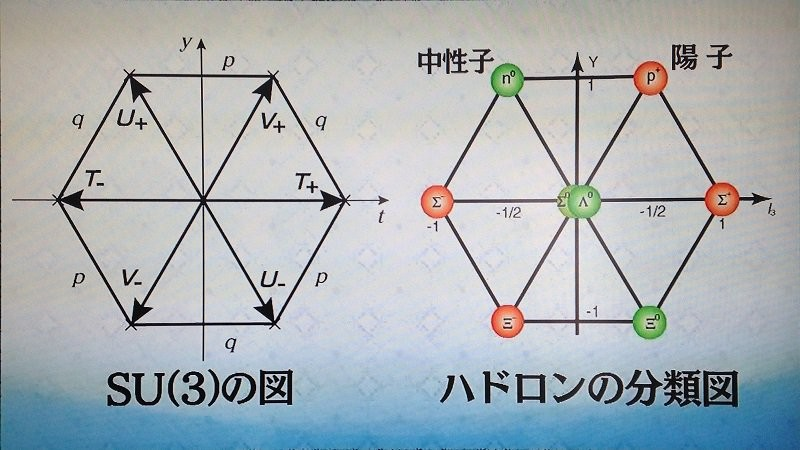
\includegraphics[width=10cm]{fig1.jpg}
\end{center}

%\newpage
\href
{https://mathtod.online/media/NFGV9VitI85F49soC6Q}
{図2}
\begin{center}
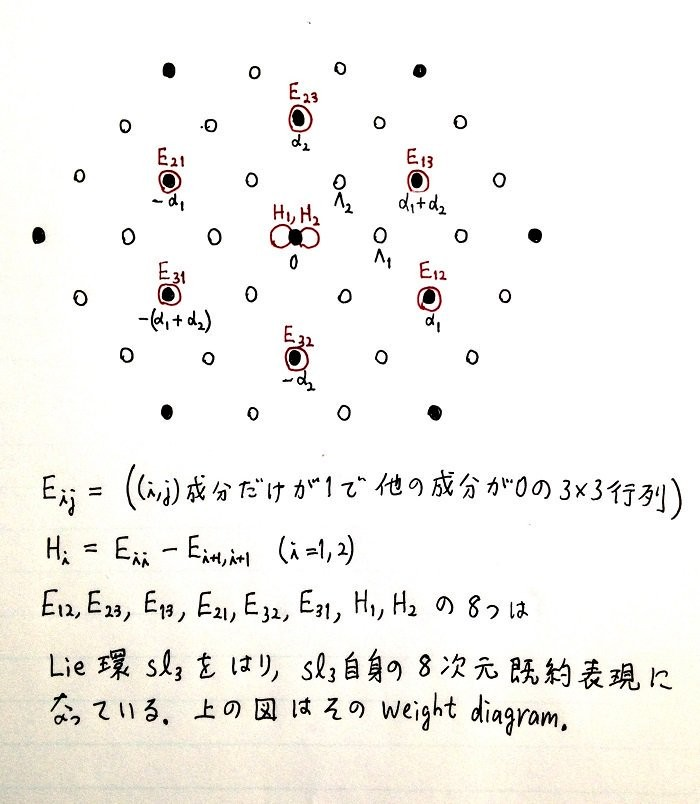
\includegraphics[width=8cm]{fig2.jpg}
\end{center}














\section{ June  1, 2017 12:02am}








黒木玄 Gen Kuroki
@genkuroki


$SU(3)$ のLie代数の複素化 $\operatorname{sl}_3(\mathbb C)$ は以下を生成元に持ちます:\begin{align*}&H_i=E_{ii}-E_{i+1,i+1},\\&E_i=E_{i,i+1},\\&F_i=E_{i+1,i}.\end{align*}ここで $i=1,2$ です. 

そして, それらは次を満たします:\begin{align*}&[H_i,H_j]=0,\\&[H_i,E_j]=a_{ij}E_j,\\&[H_i,F_j]=-a_{ij}F_j,\\&[E_i,F_j]=\delta_{ij}H_i,\\&(\ad E_i)^{1-a_{ij}}E_j=0 \quad(i\ne j),\\&(\ad F_i)^{1-a_{ij}}F_j=0 \quad(i\ne j).\end{align*}ここで\begin{align*}&(\ad A)B=[A,B],\\& [a_{ij}]=\begin{bmatrix}2&-1\\ -1&2\end{bmatrix}.\end{align*}これの証明も単なる行列の易しい計算です. 









\section{ June  1, 2017 12:09am}


黒木玄 Gen Kuroki
@genkuroki

以上の計算をがんばってすることの御利益はKac-Moody代数の定義をすぐに理解できるようになることです. 一つ前の発言の行列 $[a_{ij}]$ を
\begin{itemize}
\item サイズは $\ell$ とする. 
\item 対角成分はすべて $2$ であるとする. 
\item 非対角成分は非負の整数で, $i\ne j$ について $a_{ij}=0$ と $a_{ji}=0$ は同値であるとする. 
\end{itemize}
と一般化しましょう. 

生成元 $H_i,E_i,F_i$ ($i=1,\ldots,\ell$) と一つ前の発言に書いた形の関係式で定義されるLie代数が型 $[a_{ij}]$ のKac-Moody代数の定義です. たったこれだけ! 

「八道説」の $\operatorname{sl}_3(\mathbb C)$ での随伴表現による解釈を知っていて, その関係式も実際に自分の手で計算してよく知っていれば, Kac-Moody代数の定義は典型的に「以下同様」のスタイルになっていることを理解できるわけです. 

数学は基本的にこういうみもふたもない話なので, 聞き慣れない数学用語に何か「権威」を感じている場合にはほぼ確実に誤解していることになると思います. 









%%%%%%%%%%%%%%%%%%%%%%%%%%%%%%%%%%%%%%%%%%%%%%%%%%%%%%%%%%%%%%%%%%%%%%%%%%%%
\end{document}
%%%%%%%%%%%%%%%%%%%%%%%%%%%%%%%%%%%%%%%%%%%%%%%%%%%%%%%%%%%%%%%%%%%%%%%%%%%%
